% This file was created with tikzplotlib v0.9.12.
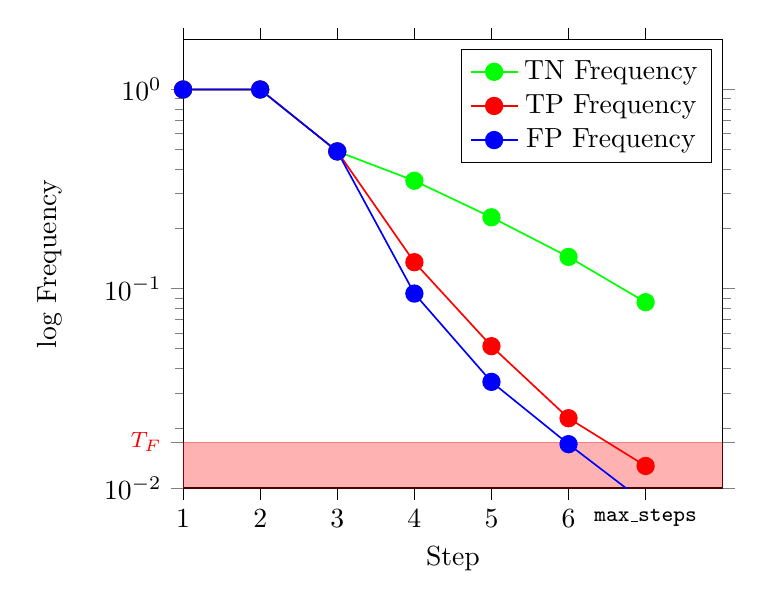
\begin{tikzpicture}

\definecolor{color0}{rgb}{0.12156862745098,0.466666666666667,0.705882352941177}

\begin{axis}[
log basis y={10},
tick align=outside,
tick pos=both,
x grid style={white!69.0196078431373!black},
xlabel={Step},
xmin=1, xmax=8,
xtick style={color=black},
xtick={1,2,3,4,5,6,7},
xticklabels={1,2,3,4,5,6,\footnotesize
\texttt{max\_steps}},
y grid style={white!69.0196078431373!black},
ylabel={$\log$ Frequency},
ymin=0.01, ymax=1.77827941003892,
ymode=log,
extra y ticks={0.017}, % Adding the specific y tick
extra y tick labels={\footnotesize $T_F$}, % Labeling it as T_F
extra y tick style={font=\footnotesize, yticklabel style={color=red}}
]
\path [draw=red, fill=red, opacity=0.3]
(axis cs:1,0.017)
--(axis cs:1,1e-05)
--(axis cs:2,1e-05)
--(axis cs:3,1e-05)
--(axis cs:4,1e-05)
--(axis cs:5,1e-05)
--(axis cs:6,1e-05)
--(axis cs:7,1e-05)
--(axis cs:8,1e-05)
--(axis cs:8,0.017)
--(axis cs:8,0.017)
--(axis cs:7,0.017)
--(axis cs:6,0.017)
--(axis cs:5,0.017)
--(axis cs:4,0.017)
--(axis cs:3,0.017)
--(axis cs:2,0.017)
--(axis cs:1,0.017)
--cycle;

\addplot [semithick, green, mark=*, mark size=3, mark options={solid}]
table {%
1 1
2 1
3 0.489
4 0.3484
5 0.2284
6 0.1444
7 0.0856
};
\addlegendentry{TN Frequency}

\addplot [semithick, red, mark=*, mark size=3, mark options={solid}]
table {%
1 1
2 1
3 0.489
4 0.1359
5 0.0515
6 0.0224
7 0.0129
};
\addlegendentry{TP Frequency}

\addplot [semithick, blue, mark=*, mark size=3, mark options={solid}]
table {%
1 1
2 1.0
3 0.489
4 0.0946
5 0.0341
6 0.0166
7 0.0084
};
\addlegendentry{FP Frequency}
\end{axis}


\end{tikzpicture}
